\chapter{Enemy Data}

\begin{definition}[Jeffrey Says]
\setlength{\intextsep}{0pt}%
\setlength{\columnsep}{3pt}%
\begin{wrapfigure}{l}{0.12\textwidth}
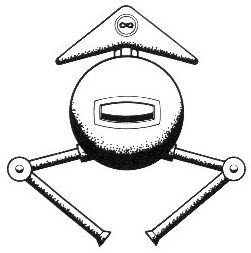
\includegraphics[width=\linewidth]{src/callout/ia.jpg} 
\end{wrapfigure}
\small
After CBM was over, I spruced up GENESYS and got it to the point where I could
  actually start doing the attack waves. That's more or less what I've been
  doing up till now: designing sprite sequences, flight paths, puzzles in some
  levels, testing 'em to make sure they are not too difficult for mere mortals.
  After doing about 40 waves and realising that there's still another 60 to go,
  'Attack Wave Fatigue' starts to show up, but you just gotta plug on and get
  'em done. At the time of writing this I've done 66 of them. I also did a lot
  of tweaking to the flight mechanics, and designed the display panel and got
  its various gauges and meters running.
\end{definition}

This section provides the level data for each wave of enemies in each
planet. Figures are provided to indicate the appearance and movement
pattern of the enemy.
\subfile{level_data/level_data_appendix}

